% Discussion (new 2026-11-11): VII-A storage against arithmetic (Fig. 10, rows 114-115 of evaluation/dac_2x2, numbers
% asserted in scripts/make_fig_storage.py); VII-B beat filling on newer DRAM (moved verbatim from the former VI-F).
\section{Discussion}
\label{sec:disc}

\subsection{Storage Versus Arithmetic in a DRAM Die}
\label{sec:disc:storage}

% P:disc-storage-claim
Filling idle beats with storage costs a DRAM die less area per unit of speed than filling them with arithmetic. We
charge each design its added logic area $\Delta A$ per unit of speed-up $S$ over stock AiM, $\Delta A / (S - 1)$.
On GEMMs of eight token rows, LP-Spec-style adds 0.655\,mm$^2$ per die for each +1$\times$ and CoDe adds 0.189,
3.5$\times$ less (Fig.~\ref{fig:storage}); on HBM2 the gap is 3.1$\times$ (0.405 against 0.130\,mm$^2$ per
pseudo-channel), and end to end, at the operating points of Section~\ref{sec:method:work}, 3.4$\times$ and
3.1$\times$.

% Fig. 10, one column, generated by scripts/make_fig_storage.py; placement checked on the float map after each build
\begin{figure}[t]
  \centering
  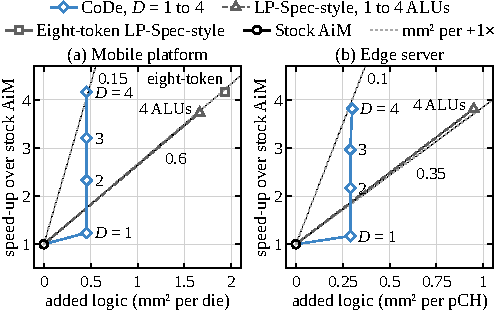
\includegraphics[width=\columnwidth]{figs/fig_storage.pdf}
  \Description{Two line charts of speed-up over stock AiM against the logic area added over stock AiM, one for the mobile platform and one for the edge server, with CoDe's points at depths one to four, a dashed LP-Spec-style segment from stock AiM to four ALUs, and stock AiM at zero added area.}
  \caption{Speed-up over stock AiM against added logic area: (a)~mobile platform; (b)~edge server.}
  \label{fig:storage}
\end{figure}

% P:disc-storage-cause
The DRAM die sets this trade. It builds logic ten times less densely than an ASIC~\cite{devaux}, so multipliers are the
costliest way to fill a beat, while its all-bank column already spans four command clocks, so a beat costs clock cycles
rather than area (Section~\ref{sec:bg:depth}). CoDe therefore pays once, for the tile's storage, gains its beats
from the PU clock and pays for those cycles in power; its peak power stays below LP-Spec-style's when both designs
gate their clocks (Section~\ref{sec:eval:energy}).

\subsection{Beat Filling on Newer DRAM}
\label{sec:disc:newdram}

% P:disc-newer-dram-depth
Beat filling extends to faster DRAM wherever the all-bank column stays at four command clocks. We evaluate
LPDDR5-6400 and HBM2 because LP-Spec~\cite{lpspec} and P3-LLM~\cite{p3llm} were built on them. JEDEC fixes
$t_\mathrm{CCD\_L}$ at $4\,t_\mathrm{CK}$ on LPDDR5~\cite{jedeclpddr5}; if LPDDR5X-9600 keeps it, its 1.2\,GHz command
clock~\cite{micronlp5x} gives a 3.33\,ns column. HBM3 at 6.4\,Gb/s runs its command clock at 1.6\,GHz~\cite{synopsyshbm3};
at HBM2's four-clock column (Table~\ref{tab:params}), its column lasts 2.5\,ns\ASSUMPTION. On either memory a PU at CK
still runs $D = 4$ beats per column, CoDe's tile fills them, and \UMAC stays at 1 while the MAC rate grows.

% P:disc-newer-dram-clock
Such a PU runs above 1\,GHz, and DRAM silicon is moving toward it: LPDDR5X-9600 already clocks its data path at four
times CK~\cite{micronlp5x}, DRAM periphery is adopting high-k metal gates~\cite{skhynixhkmg,micron1gamma},
TSMC~\cite{tsmchbm4} plans to build HBM4 base dies in its 12-nm and 5-nm logic processes, and Samsung's
LPDDR5X-PIM~\cite{lp5xpim} already computes inside the newer generation.
